\chapter{Chapter 1}
\label{Chp:1}

\section{Introduction}

Studying the brain is a profoundly complex challenge. With approximately $10^{11}$ neurons, each forming around $10^{3}$ synaptic connections---yielding a staggering total of roughly $10^{14}$ connections---a whole-brain analysis at single-neuron resolution remains computationally intractable\footnote{At least with currently available computational power.}. To navigate this complexity, computational neuroscience has emerged as an interdisciplinary field that relies on advanced mathematical models and simulation tools to decode brain dynamics.

For medium-to large-scale analyses, researchers typically employ coarse-grained models. Rather than resolving the microscopic details of individual cells, these models adopt more complex structures, such as entire neural populations, as their fundamental units. The resulting macroscopic or mesoscopic dynamics can then be validated against empirical data from functional imaging, such as fMRI or EEG.

Despite the necessity of these large-scale abstractions, single-neuron ionic models remain indispensable. A microscopic understanding of neural dynamics is not only of fundamental scientific interest in its own right, but it also serves as the rigorous foundation from which accurate coarse-grained models can be mathematically derived.
\newline
We will now analyze two prominent ionic models and use one of them on a network setup in order to describe larger spatial areas.

%Aggiungere un riferimento bibliografico?

\section{The Hodgkin-Huxley model}
One of the most prominent ionic models is the Hodgkin-Huxley (HH) model. It was first introduced by Alan Hodgkin and Andrew Huxley in 1952 \cite{hodgkin1952quantitative}, who received the 1963 Nobel Prize in Physiology or Medicine for this work.
\newline
It leverages a system of nonlinear ordinary differential equations that describes the generation and propagation of action potentials in neurons. The model simulates the dynamics of the membrane potential $V(t)$ as a function of the ionic currents crossing the cell membrane: a sodium current ($Na^+$), a potassium current ($K^+$), and a leakage current ($L$).

The system is governed by the following equation for the potential:

\begin{equation}
    C_{m}\frac{dV}{dt} = -(g_{Na}m^{3}h(V-V_{Na}) + g_{K}n^{4}(V-V_{K}) + g_{L}(V-V_{L})) + I_{app}
    \label{eq:HH_voltage}
\end{equation}

where $C_m$ is the membrane capacitance, $g_i$ are the maximum conductances, and $V_i$ are the reversal potentials for the respective ion channels. $I_{app}$ represents the applied external current.

The gating variables $m$, $h$, and $n$ represent the probability for each ionic species to pass through the cellular membrane and they evolve according to the following first-order differential equations:

\begin{equation}
    \begin{aligned}
        \frac{dm}{dt} &= \alpha_{m}(V)(1-m) - \beta_{m}(V)m \\
        \frac{dh}{dt} &= \alpha_{h}(V)(1-h) - \beta_{h}(V)h \\
        \frac{dn}{dt} &= \alpha_{n}(V)(1-n) - \beta_{n}(V)n
    \end{aligned}
    \label{eq:HH_gating}
\end{equation}


The voltage-dependent transition rates $\alpha_i(V)$ and $\beta_i(V)$ are empirically determined functions of the membrane potential, given by the following equations:

\begin{equation}
    \begin{aligned}
        \alpha_{m}(V) &= \frac{0.1(V+50)}{1 - \exp\left(-\frac{V+50}{10}\right)} \\[2ex]
        \alpha_{h}(V) &= 0.07 \exp\left(-\frac{V+75}{20}\right) \\[2ex]
        \alpha_{n}(V) &= \frac{0.01(V+65)}{1 - \exp\left(-\frac{V+65}{10}\right)}
    \end{aligned}
    \qquad\qquad
    \begin{aligned}
        \beta_{m}(V) &= 4 \exp\left(-\frac{V+75}{18}\right) \\[2ex]
        \beta_{h}(V) &= \frac{1}{1 + \exp\left(-\frac{V+45}{10}\right)} \\[2ex]
        \beta_{n}(V) &= 0.125 \exp\left(-\frac{V+75}{80}\right)
    \end{aligned}
    \label{eq:HH_rates}
\end{equation}

For the numerical simulations, reported for instance in Figure \ref{fig:hh_dynamics}, the parameters described in \cite{centofanti2024cma} were adopted: $C_m = 1 \, \mu\text{F/cm}^2$, $V_{Na} = 40 \, \text{mV}$, $V_{K} = -87 \, \text{mV}$, $V_{L} = -64.387 \, \text{mV}$, $g_{Na} = 120 \, \text{mS/cm}^2$, $g_{K} = 36 \, \text{mS/cm}^2$, $g_{L} = 0.3 \, \text{mS/cm}^2$ and the initial conditions: $V_0= -75 \text{mV}$, $n_0=0.317$, $m_0=0.05$, $h_0=0.595$.
Since a single neuron is not isolated it is interesting to analyze its response to external currents.

\subsection*{Asymptotic behavior}
The behavior of the HH model in response to a constant applied current $I_{app}$ exhibits distinct phase transitions depending on the stimulus intensity \cite{centofanti2024cma}:

\begin{itemize}
    \item \textbf{Quiescent regime} ($I_{app} \lesssim 2.21 \, \mu\text{A/cm}^2$):
    For current values below the critical threshold, the system has a unique stable equilibrium point corresponding to the resting potential. The neuron does not generate repetitive spikes.
    
    \item \textbf{Repetitive firing} ($2.21 \lesssim I_{app} \lesssim 150 \, \mu\text{A/cm}^2$):
    Once the threshold of $2.21 \, \mu\text{A/cm}^2$ is exceeded, the equilibrium point loses stability (Hopf bifurcation) and the system is attracted to a stable limit cycle. In this regime, the neuron discharges continuous trains of action potentials.
    
    \item \textbf{Depolarization block} ($I_{app} \gtrsim 150 \, \mu\text{A/cm}^2$):
    For extremely high currents, the limit cycle disappears and the system stabilizes again at a high-voltage fixed point (stable depolarized state), ceasing to oscillate.
\end{itemize}

This model is realistic, but somewhat convoluted for our objectives. In fact, our primary aim (as discussed by subsequent chapters) is to simulate a network of neurons and emulate it through Machine Learning (ML). To this end, we need a system that is as simple as possible, while it exhibits, like a physically realistic neuron, oscillations for currents that exceed a critical threshold.

\begin{figure}[htbp]
    \centering
    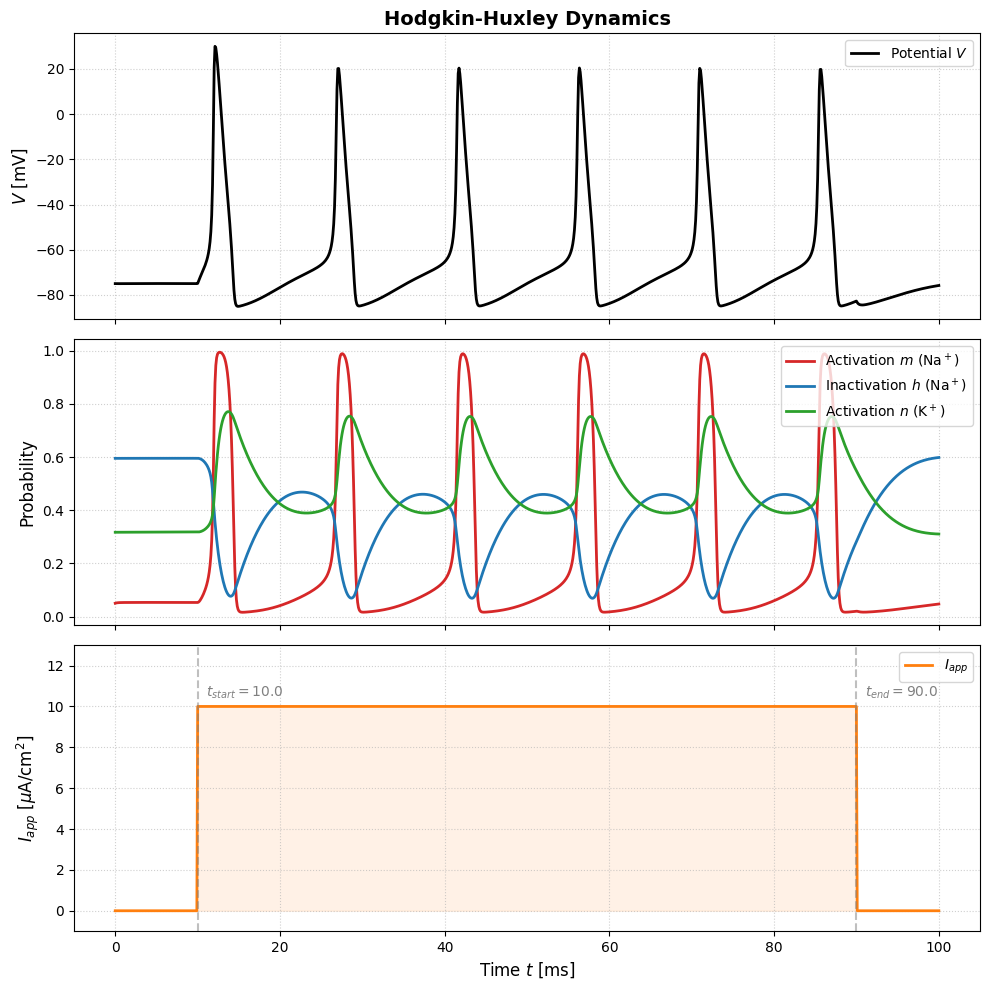
\includegraphics[width=\textwidth]{img/FH_model/HH_dynamics.png}
    \caption{Simulated dynamics of the Hodgkin-Huxley model. The plots illustrate the temporal evolution of the transmembrane potential $V$ along with the gating variables $m, h$, and $n$ under the influence of an applied external current $I_{app}(t)$.}
    \label{fig:hh_dynamics}
\end{figure}

\newpage
\section{The FitzHugh-Nagumo model}
The FitzHugh-Nagumo (FH) model \cite{centofanti2024comconf} is a two-dimensional simplification of the HH model that preserves the essential characteristics of excitability. The dynamical equations for the fast variable $V$ (potential) and the slow variable $w$ (recovery) are:

\begin{equation}
    \begin{aligned}
        \frac{dV}{dt} &= bV(V-\beta)(\delta-V) - cw + I_{app} \\
        \frac{dw}{dt} &= \epsilon(V - \gamma w)
    \end{aligned}
    \label{eq:FHN}
\end{equation}

The parameters used in all the FH simulations throughout this thesis are $b = 5$, $c = 1$, $\beta = 0.1$, $\delta = 1$, $\epsilon = 0.1$, $\gamma = 0.25$ \cite{centofanti2024comconf}.

\subsection*{Asymptotic behavior}
\label{sec:FHN_dynamics}
The dynamics of the FHN system depends on the value of $I_{app}$, which vertically translates the cubic nullcline, modifying the position and stability of the fixed point:

\begin{itemize}
    \item \textbf{Stable equilibrium regime ($I_{app} \lesssim 0.2$):} 
    The system presents a unique stable fixed point located on the left branch of the cubic nullcline (near the resting state). For small stimuli, the system returns to equilibrium without generating oscillations.
    
    \item \textbf{Oscillatory regime ($0.2 \lesssim I_{app} \lesssim 2.1$):} 
    When the current exceeds the first critical threshold ($I_{th1} \approx 0.21$), the fixed point enters the unstable region of the nullcline (between the two knees of the cubic). The equilibrium loses stability and a stable limit cycle emerges. The system produces sustained periodic oscillations, as highlighted in Figure \ref{fig:fhn_time_series} - \ref{fig:fhn_phase_space}.
    
    \item \textbf{Saturation regime ($I_{app} \gtrsim 2.1$):} 
    Increasing the current beyond the second critical threshold ($I_{th2} \approx 2.1$), the intersection of the nullclines shifts to the stable right branch. The limit cycle vanishes, and the system stabilizes at a high-potential equilibrium (permanent excited state).
\end{itemize}

\begin{figure}[H]
    \centering
    \begin{minipage}[b]{0.58\textwidth}
        \centering
        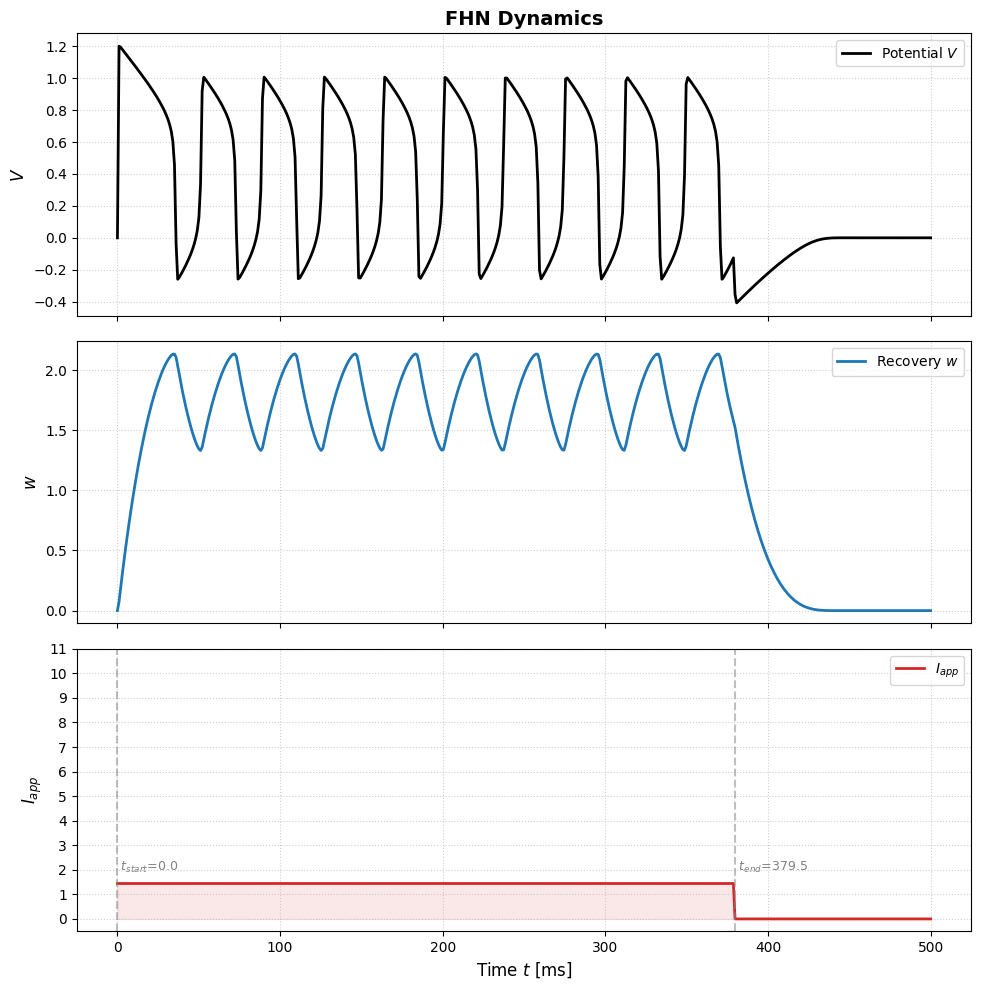
\includegraphics[width=\textwidth]{img/FH_model/No_Network/limit_cycle.png}
        \caption{Time evolution of $V$ and $w$ in the oscillatory regime.}
        \label{fig:fhn_time_series}
    \end{minipage}
    \hfill
    \begin{minipage}[b]{0.38\textwidth}
        \centering
        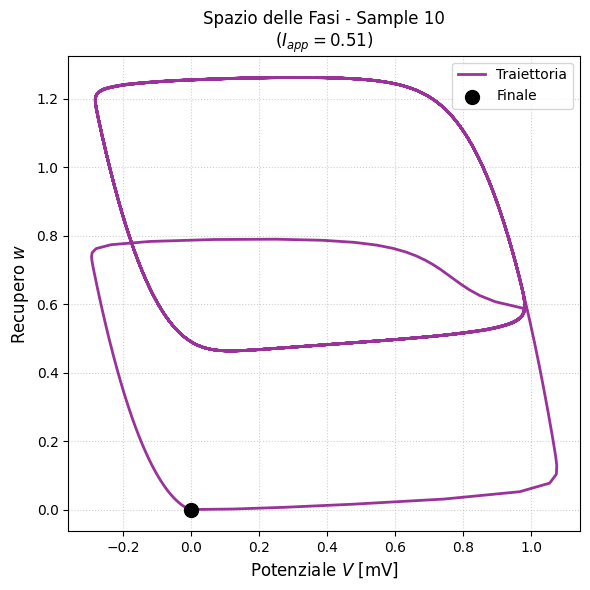
\includegraphics[width=\textwidth]{img/FH_model/No_Network/limit_cycle_phase_space.png}
        \caption{Trajectory in the phase plane $(V, w)$.}
        \label{fig:fhn_phase_space}
    \end{minipage}
    \caption*{Dynamics of the FitzHugh-Nagumo model with $I_{app} \approx 1.44$ (left: space-time, right: phase space). After a transient the system exhibits a stable limit cycle. Note that since the perturbation (bottom left) is a square wave once it goes off the system returns to the only stable equilibrium $(0,0)$.}
    \label{fig:fhn_dynamics}
\end{figure}


In Fig \ref{fig:fhn_time_series} we can see a response of the system to a square wave perturbation. In particular, we observe an oscillatory dynamics while the external current is on.
Since our ML analysis (chapter \ref{Chpt3}) is based on mapping  functions (perturbations) to functions (responses), we considered the square wave perturbation class as it provides an easy-to-study function basis

Starting from these premises, we turned to study the spatial extension of the FH model and analyzed its response to a square wave perturbation localized in space (i.e. applied to a single node).


\newpage
\section{From single neuron to spatially extended systems}
\label{sec:extended_network}
The framework discussed thus far has focused on the dynamics of an isolated single node. In order to transition from a microscopic to a mesoscopic description of neural dynamics, we embedded the FitzHugh-Nagumo (FHN) model within a network topology. Our primary objective was to investigate whether the resulting high-dimensional system of ordinary differential equations (ODEs) could be effectively approximated by a single neural operator trained via deep learning techniques, which will be detailed in Chapter \ref{Chp:2}.

To this end, we considered a spatially extended system characterized by a specific input-output mapping. An external stimulus, modeled as a square-wave current, was injected into a designated \textcolor{blue}{\textbf{input node}}. The signal then propagated through the network via diffusive coupling, while each node underwent local reaction dynamics governed by the FHN equations. Finally, the response of the system was recorded by extracting the membrane potential of a designated \textcolor{red}{\textbf{output node}}. This setup is illustrated by two examples in Figure \ref{fig:fh_comparison}.


Formally, let $\mathcal{G} = (\mathcal{V}, \mathcal{E})$ be an unweighted graph representing the neural network topology. The diffusive coupling between neurons are modeled using the elements $L_{ij}$ of the graph Laplacian matrix $\mathbf{L} = \mathbf{D}_{deg} - \mathbf{A}$, where $\mathbf{D}_{deg}$ is the diagonal degree matrix and $\mathbf{A}$ is the adjacency matrix. The elements of the Laplacian are explicitly defined as:
\begin{equation}
L_{ij} = 
\begin{cases} 
\text{deg}(i) & \text{if } i = j \\
-1 & \text{if } (i,j) \in \mathcal{E} \\
0 & \text{otherwise}
\end{cases}
\end{equation}

The dynamics of the coupled system are therefore governed by the following set of equations for each node $i \in \mathcal{V}$:
\begin{equation}
\label{eq:coupled_FHN}
\begin{aligned}
\frac{dV_i}{dt} &= b V_i (V_i - \beta)(\delta - V_i) - c w_i + I_{app, i}(t) - \sigma \sum_{j=1}^{|\mathcal{V}|} L_{ij} V_j \\
\frac{dw_i}{dt} &= \epsilon (V_i - \gamma w_i)
\end{aligned}
\end{equation}
where the coefficient $\sigma$ modulates the global coupling strength (i.e., the intensity of diffusion) across the network.
\begin{figure}[htbp]
    \centering
    % --- Prima immagine (sopra) ---
    \begin{subfigure}[b]{1.0\textwidth}
        \centering
        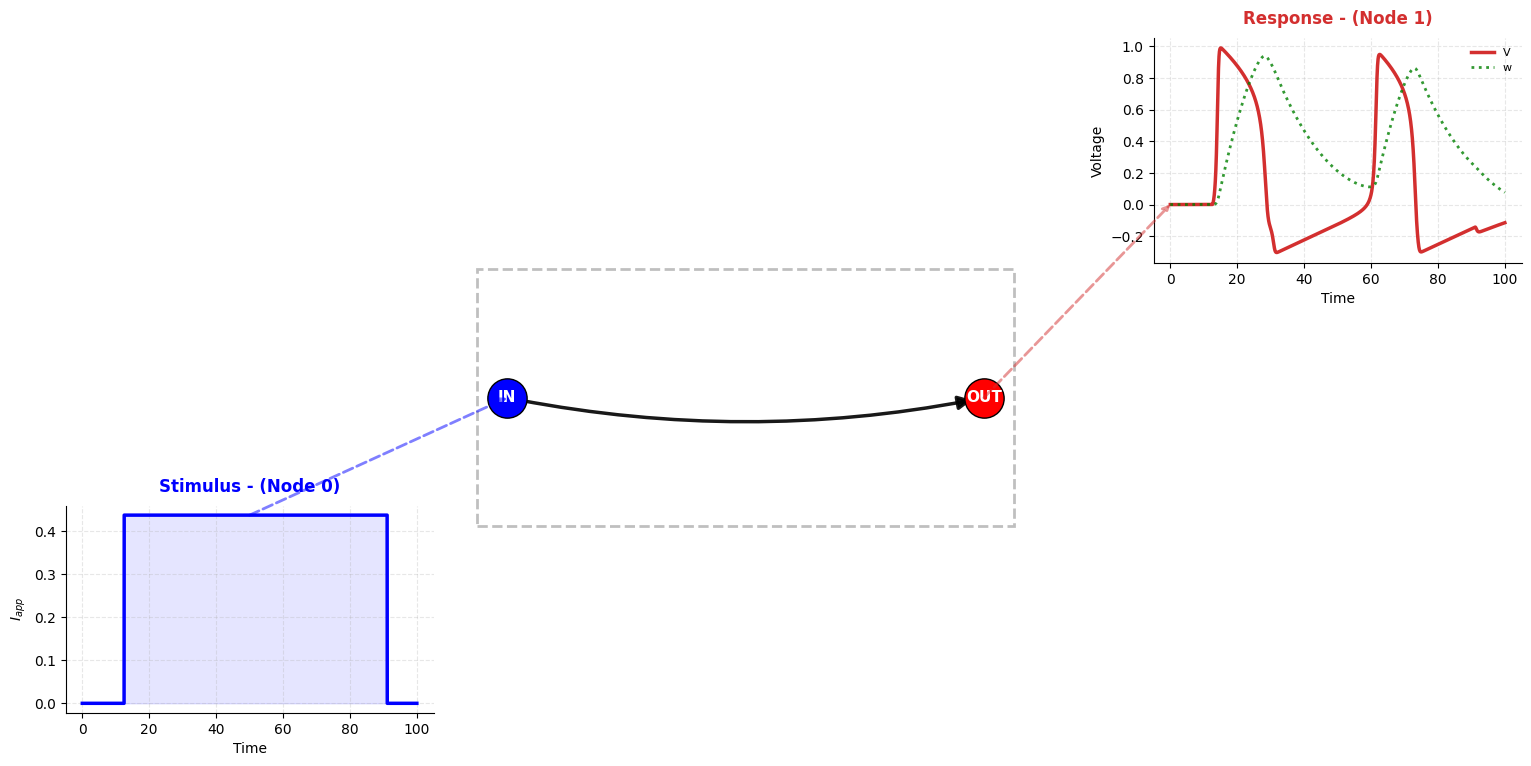
\includegraphics[width=\textwidth]{img/FH_model/1to2/output0to1_v2.png}
        \caption{Minimal setup: Input $\rightarrow$ Output}
        \label{fig:fh_output}
    \end{subfigure}
    
    \vspace{0.5cm} % Spazio verticale tra le due figure
    
    % --- Seconda immagine (sotto) ---
    \begin{subfigure}[b]{1.0\textwidth}
        \centering
        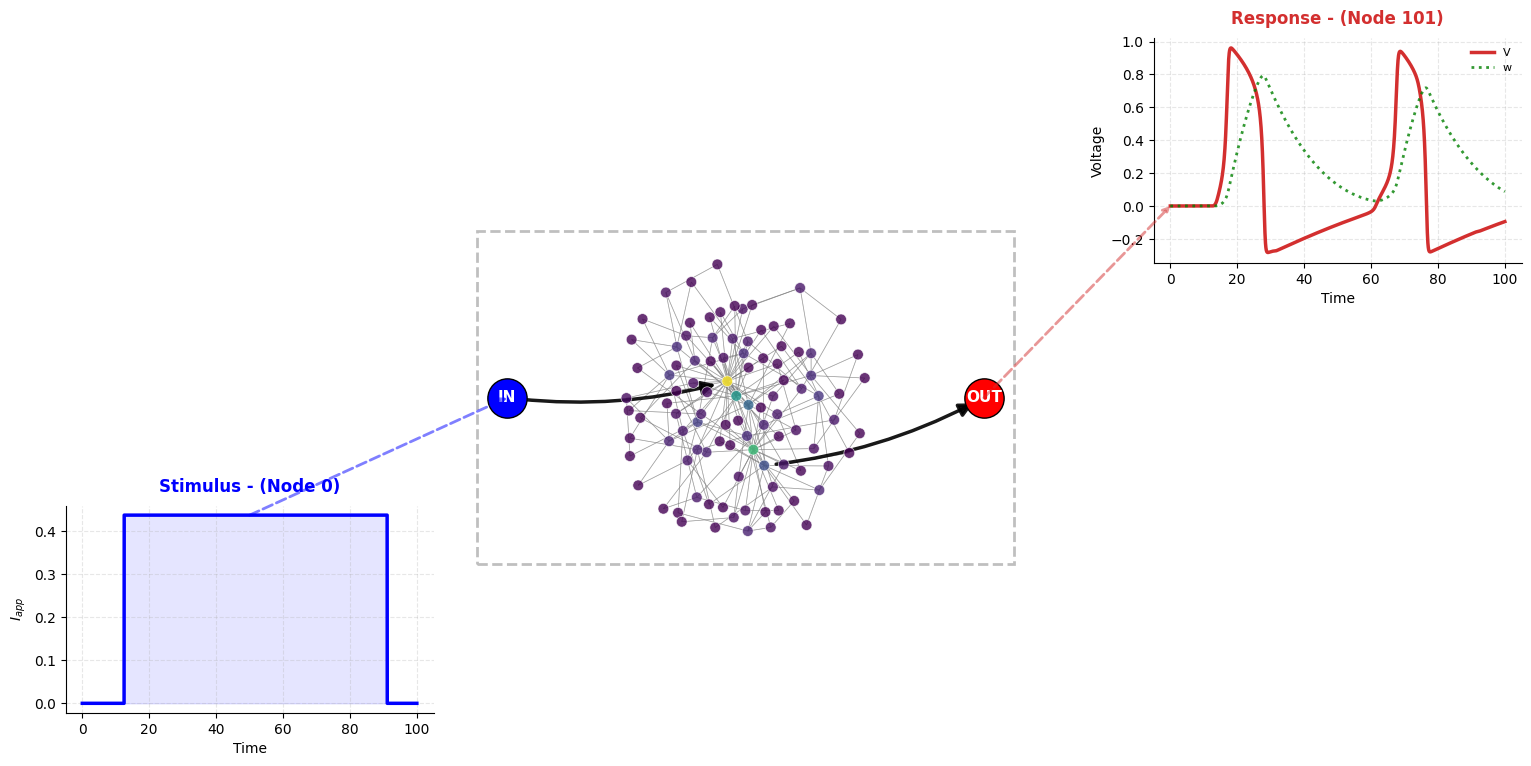
\includegraphics[width=\textwidth]{img/FH_model/BA_Network/network_plot_BA_N=100_v2.png}
        \caption{Extended topology: Input $\rightarrow$ Network $\rightarrow$ Output}
        \label{fig:fh_dynamics}
    \end{subfigure}
    
    \caption{Schematic representation of the network setup. (a) A minimal configuration illustrating the direct signal transmission from an input to an output node. (b) A more complex topology utilizing a Barabási-Albert (BA) scale-free network ($N=100$, $m=2$), demonstrating how the input stimulus propagates through a mesoscopic structure before reaching the output node.}
    \label{fig:fh_comparison}
\end{figure}

Having established the mathematical formulation of the coupled system, in the next chapter we will introduce the principles of Scientific Machine Learning (SciML). Specifically, we will focus on the operator learning techniques employed to emulate the input-output mapping of the spatially extended system—that is, predicting the continuous temporal evolution of the \textcolor{red}{\textbf{output node}}'s potential as a direct consequence of a specific perturbation applied to the \textcolor{blue}{\textbf{input node}}.
